

\documentclass[twoside,twocolumn]{article}

\usepackage{blindtext} % Package to generate dummy text throughout this template 
\usepackage{graphicx}
\usepackage[sc]{mathpazo} % Use the Palatino font
\usepackage[T1]{fontenc} % Use 8-bit encoding that has 256 glyphs
\linespread{1.05} % Line spacing - Palatino needs more space between lines
\usepackage{microtype} % Slightly tweak font spacing for aesthetics

\usepackage[english]{babel} % Language hyphenation and typographical rules

\usepackage[hmarginratio=1:1,top=32mm,columnsep=20pt]{geometry} % Document margins
\usepackage[hang, small,labelfont=bf,up,textfont=it,up]{caption} % Custom captions under/above floats in tables or figures
\usepackage{booktabs} % Horizontal rules in tables

\usepackage{lettrine} % The lettrine is the first enlarged letter at the beginning of the text

\usepackage{enumitem} % Customized lists
\setlist[itemize]{noitemsep} % Make itemize lists more compact

\usepackage{abstract} % Allows abstract customization
\renewcommand{\abstractnamefont}{\normalfont\bfseries} % Set the "Abstract" text to bold
\renewcommand{\abstracttextfont}{\normalfont\small\itshape} % Set the abstract itself to small italic text

\usepackage{titlesec} % Allows customization of titles
\renewcommand\thesection{\Roman{section}} % Roman numerals for the sections
\renewcommand\thesubsection{\roman{subsection}} % roman numerals for subsections
\titleformat{\section}[block]{\large\scshape\centering}{\thesection.}{1em}{} % Change the look of the section titles
\titleformat{\subsection}[block]{\large}{\thesubsection.}{1em}{} % Change the look of the section titles

\usepackage{fancyhdr} % Headers and footers
\pagestyle{fancy} % All pages have headers and footers
\fancyhead{} % Blank out the default header
\fancyfoot{} % Blank out the default footer
\fancyhead[C]{Titulo $\bullet$ Junio 2019 $\bullet$ } % Custom header text
\fancyfoot[RO,LE]{\thepage} % Custom footer text

\usepackage{titling} % Customizing the title section

\usepackage{hyperref} % For hyperlinks in the PDF

%----------------------------------------------------------------------------------------
%	TITLE SECTION
%----------------------------------------------------------------------------------------

\setlength{\droptitle}{-4\baselineskip} % Move the title up

\pretitle{\begin{center}\Huge\bfseries} % Article title formatting
\posttitle{\end{center}} % Article title closing formatting
\title{Comparación Bases de datos NoSQL} % Article title
\author{Andre Reinoso, Samuel Nuñez, Andres De la Barra ,David Damian y Richard Cruz}
\date{\today} % Leave empty to omit a date
\renewcommand{\maketitlehookd}{%
\begin{abstract}
\noindent Ingles
\end{abstract}
\begin{abstract}
\noindent Español.
\end{abstract}
}

%----------------------------------------------------------------------------------------

\begin{document}

% Print the title
\maketitle

%----------------------------------------------------------------------------------------
%	ARTICLE CONTENTS
%----------------------------------------------------------------------------------------

\section{Introduccion}
\lettrine[nindent=0em,lines=3]{L}as bases de datos son una de las tecnologías para la organización de la información más eficientes y poderosas de que disponemos en la actualidad. De hecho, las bases de datos están en el núcleo de los sistemas y de los servicios de información que poseen mayor significación tanto desde un punto de vista económico como social. Por ejemplo, la mayor parte de los sistemas de información empresarial, desde el control de existencias de almacén hasta el sistema de ventas, tiene en su núcleo una base de datos. En el seno de muchas actividades sociales vinculadas con la gestión del conocimiento sucede otro tanto: desde la gestión de archivos y museos hasta la automatización de centros de documentación, pasando por los mejores servicios de información en Internet o por la gestión de investigaciones académicas, todos estos sistemas tienen una base de datos en su núcleo. En el presente articulo se desarrollara el tema de bases de datos NoSQL.


%------------------------------------------------

\section{Objetivos}

\begin{itemize}
\item Entender qué es una máquina virtual.
\item Entender qué es un contenedor.
\item Comparar ambos conceptos.
\item Establecer un juicio acerca de las ofertas y el potencial de ambas.

\end{itemize}




%------------------------------------------------

\section{Desarrollo}

\subsection{¿Que es una maquina virtual?}

Una máquina virtual 

\begin{center}
	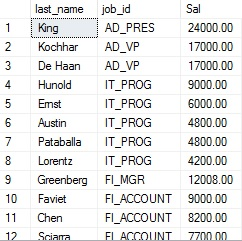
\includegraphics[width=5cm]{./Imagenes/virtualizacion} 
	\end{center}

\subsection{Insercion de datos y Consultas de datos.}
En este caso haremos la insercion de datos y consultas en MongoDb instalado en Docker.
\begin{itemize}
\item Como primer paso, se debe realizar la conexion de MongoDb:\\
docker exec -it my-mongodb mongo
\begin{center}
	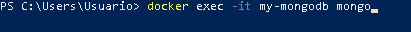
\includegraphics[width=7cm]{./Imagenes/ins1} 
	\end{center}
\item Seguidamente crearemos la colección "Base De Datos2", Despues insertaremos los datos a nuestra coleccion:\\
db.createCollection('basededatos')  
\begin{center}
	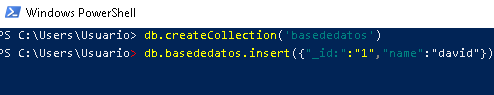
\includegraphics[width=7cm]{./Imagenes/ins2} 
	\end{center}

\item Por ultimo vamos a consultar u obtener todo los datos con el siguiente codigo:\\

\begin{center}
	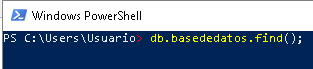
\includegraphics[width=7cm]{./Imagenes/ins3} 
	\end{center}
\end{itemize} 
\subsection{Documental}
Cuando hablamos de bases de datos documentales, nos referimos a un conjunto de información estructurada en registros y almacenada en un soporte electrónico legible desde un ordenador. Cada uno de los registros compone una unidad autónoma de información que puede estar a su vez estructurada en diferentes campos o tipos de datos que se almacenan en dicha base de datos. Por ejemplo, entre los campos se pueden encontrar: nombre del documento, título, palabras clave que caracterizan el tema tratado en el documento, fecha o autor. Para cada uno de los documentos que componen la base de datos es necesario hacer un registro, de esta manera, se puede recuperar dicho registro y determinado documento.

\begin{center}
	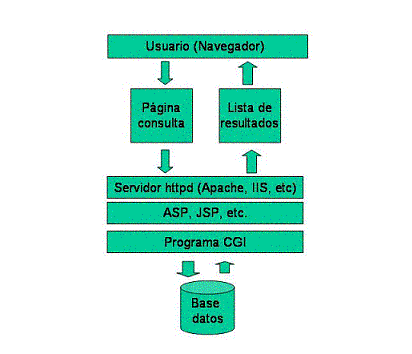
\includegraphics[width=7cm]{./Imagenes/documental} 
\end{center}


Una base de datos documental utiliza documentos como la estructura para almacenamiento y consultas. En este caso, el término "documento" puede referirse a un documento de texto, pero comúnmente también puede un archivo de XML o JSON. En lugar de columnas con nombres y tipos de datos que se utilizan en una base de datos relacional, un documento contiene una descripción del tipo de datos y el valor de esa descripción.
\\
	\textbf{Tipos de bases de datos documentales:}
\begin{itemize}	

	\item Bases de datos a texto completo
	\item Bases de datos referenciales
	\item Multidisciplinares
	\item Especializadas
	\item Bases de datos de acceso local
	\item Bases de datos en CD ROM
\item Bases de datos en línea
\end{itemize} 

	\textbf{Ventajas:}
\\
Hoy en día las empresas tienen que trabajar con una gran cantidad de documentación y es muy complicado gestionar todos los documentos diarios que se generan. Por este motivo, ahora más que nunca, es imprescindible contar con un sistema de bases de datos documental en la empresa. Estas son algunas de las ventajas que aporta el uso de las bases de datos documentales:
\begin{itemize}	

	\item Capaces de almacenar cualquier tipo de información en forma de texto.
	\item Facilidad de poder manejar una gran cantidad de información, de forma rápida y en muy poco tiempo.
	\item Aumenta el rendimiento general de la empresa al poder recuperar los documentos de forma ágil y fácil.
	\item Poseen un lenguaje de consulta fácil e intuitivo.
	\item Capaz de manejar una gran cantidad de datos.
	\item Escalabilidad y ahorro de espacio.

\end{itemize} 



\subsection{Clave - Valor}
Una base de datos clave-valor es un tipo de base de datos no relacional que utiliza un método simple de clave-valor para almacenar datos. Una base de datos clave-valor almacena datos como un conjunto de pares clave-valor en los que una clave sirve como un identificador único. Tanto las claves como los valores pueden ser cualquier cosa, desde objetos simples hasta objetos compuestos complejos. Las bases de datos clave-valor son altamente divisibles y permiten el escalado horizontal a escalas que otros tipos de bases de datos no pueden alcanzar.
Las claves pueden ser organizadas por grupos clave lógicos, requiriendo solamente estas claves para ser únicas dentro de su propio grupo. Esto permite tener claves idénticas en diferentes grupos lógicos.Algunas implementaciones del almacén de valores clave proporcionan mecanismos de almacenamiento en el caché, lo que mejora en gran medida su rendimiento.
\begin{center}
	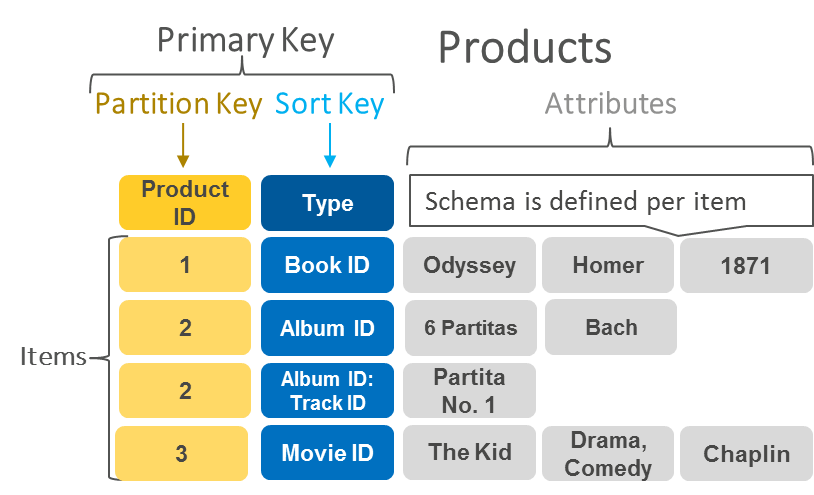
\includegraphics[width=7cm]{./Imagenes/clavevalor} 
\end{center}


Sus principales ventajas son 3: simplicidad, eficiencia y flexibilidad, que permiten unas búsquedas rápidas en lecturas a toda la BBDD, así como funciones de agregación efectivas. Por otro lado, la simplicidad también marcará sus principales inconvenientes: al carecer de estructura no es posible lanzar consultas mediante queries, y solo lo constan de una colección, complicado la implementación modelos complejos.


\subsection{Grafos}

Las bases de datos NoSQL en grafo permiten representar los datos utilizando estructuras de grafos. Un grafo es una representación abstracta de un conjunto de objetos. Los objetos de los grafos se representan mediante vértices (también llamados nodos) y aristas.

\begin{center}
	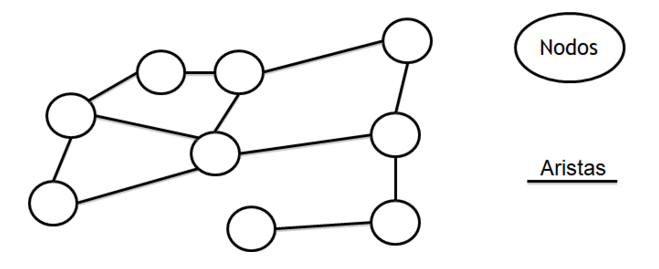
\includegraphics[width=7cm]{./Imagenes/nodos_aristas} 
\end{center}

El modelo en grafo es útil cuando los datos a almacenar tienen multitud de interrelaciones entre sí, y cuando la importancia recae más en las interrelaciones que se establecen entre los datos, que en los propios datos en sí. 
\\
En consecuencia, este tipo de bases de datos tiende a almacenar pocos datos de los objetos del mundo real que se desean representar pero muchos datos sobre sus interrelaciones, a diferencia de lo que acostumbra a suceder en las bases de datos relacionales, donde hay muchos datos de los objetos (representados mayoritariamente en las propiedades o atributos de las relaciones) y pocas interrelaciones entre los objetos (representadas mediante claves foráneas). 


\begin{itemize}
\item Ejemplo
\\ A continuación podemos ver un ejemplo simple en el que hemos creado un grafo con dos tweets (en color verde) y dos usuarios de Twitter (en color azul). Como vemos, los tweets y los usuarios se han etiquetado con las etiquetas “Tweet” y “TwitterUser” para indicar su tipo. Vemos también que uno de los tweets es un reply (se indica mediante una relación con una etiqueta “Reply”) y que los dos usuarios de Twitter se siguen mútuamente (se indica mediante la etiqueta “Follows”). También se indican los autores de cada tweet (mediante la etiqueta “Author”).


\begin{center}
	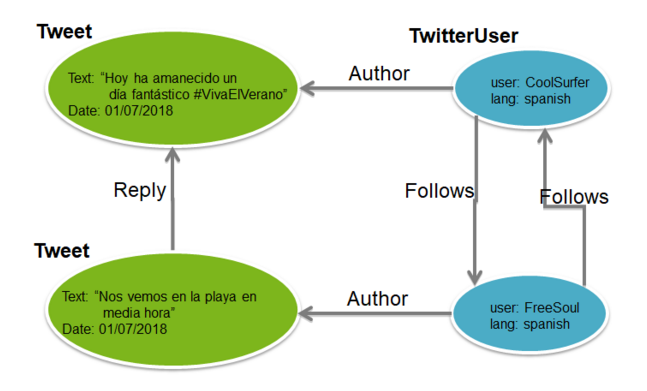
\includegraphics[width=7cm]{./Imagenes/tweet} 
\end{center}

\end{itemize} 

\subsection{Column-Store}
Es un tipo de base de datos que almacena datos utilizando un modelo orientado a columnas.
\\
\\
	\textbf{Tambien denominadas:}
\begin{itemize}	

	\item Column database
	\item Column family database
	\item Column oriented database
	\item Wide column store
	\item Columnar database
	\item Columnar store
\end{itemize} 
Utilizan un concepto llamado  keyspace . Un keyspace es algo así como un  esquema en el modelo relacional. El keyspace contiene todas las Column Family (tipo de tablas similares  en el modelo relacional), que contienen filas, que contienen columnas.
\\
\\
\textbf{Keyspace}
\begin{center}
	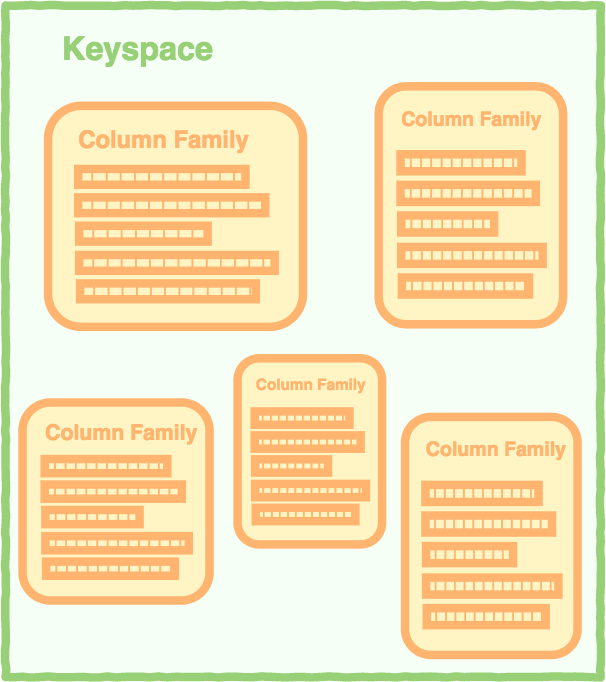
\includegraphics[width=7cm]{./Imagenes/keyspace} 
\end{center}

\textbf{Column Family}
\begin{center}
	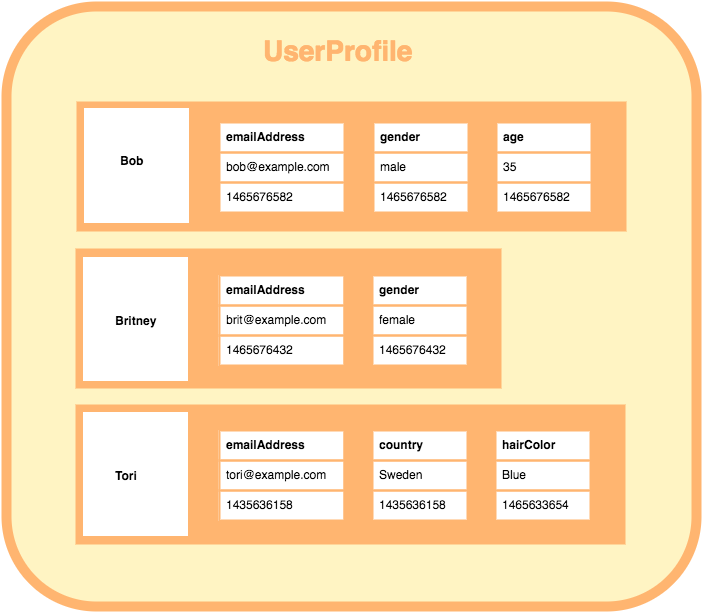
\includegraphics[width=7cm]{./Imagenes/columfamily} 
\end{center}

\begin{itemize}	

	\item Cada fila  puede contener un número diferente de columnas a las otras filas. Y las columnas no tienen que coincidir con las columnas de las otras filas (es decir, pueden tener diferentes nombres de columnas, tipos de datos, etc.).
	\item Cada columna  está contenida en su fila. No abarca todas las filas como en una base de datos relacional. Cada columna contiene un par de nombre / valor, junto con una marca de tiempo

\end{itemize} 

\textbf{Construccion de una fila}
\begin{center}
	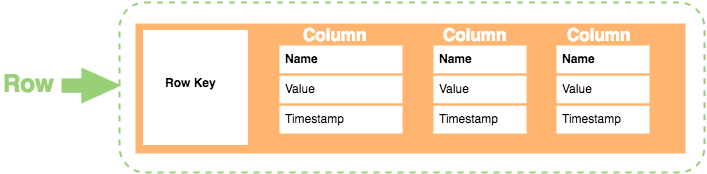
\includegraphics[width=7cm]{./Imagenes/row} 
\end{center}
\begin{itemize}	

	\item \textbf{Row Key:} Cada fila tiene una clave única, que es un identificador único para esa fila.
	\item \textbf{Column:} Cada columna contiene un nombre, un valor y una marca de tiempo.
	\item \textbf {Name:} Este es el nombre del par name/value.
	\item \textbf{Value:} Este es el valor del par name/value.
	\item \textbf{Timestamp:} Esto proporciona la fecha y la hora en que se insertaron los datos. Esto se puede utilizar para determinar la versión más reciente de los datos.
\end{itemize} 

\subsection{Comparando tipos de base de datos  NoSQL}
Más allá de las ventajas y desventajas que podamos encontrar en los tipos de bases de datos NoSQL, creemos que cada tipo de base de datos se puede aprovechar de una forma especial para un fin determinado. \\
Un grupo de ingenieros se reunieron para estudiar una comparación de calidad entre tres bases de datos populares de distintos tipos (Redis, Neo4j y MongoDB) aplicando un caso de uso real para cada tipo. El objetivo de ellos era el de evaluar las diferencias inherentes entre las bases de datos al definir los datos. \\
De acuerdo con la comparación que hicieron, pudieron inferir los siguientes hallazgos:

\begin{itemize}	
	\item Las basadas en grafos están diseñadas para ser adecuadas para representar datos fuertemente vinculados y relaciones intensivas como redes sociales, datos geográficos y bioinformática.
	\item Las basadas en documentos son adecuadas para administrar colecciones con relaciones abstractas.
	\item Las basadas en clave-valor son adecuadas cuando las relaciones no son un problema, como recuperar información sobre los nombres de productos favoritos de los clientes, los carritos de la compra y la sesión de un usuario.
	\item Se puede considerar la combinación de más de un tipo de base de datos para cumplir con más de uno de los objetivos anteriores
\end{itemize}

Ellos encontraron que las bases de datos basadas en grafos eran la mejor opción cuando se trataba de relaciones intensivas. Las bases de datos basadas en documentos eran mejor cuando se trataba de colecciones y relaciones abstractas. Finalmente, las bases de datos clave-valor eran las mejores cuando las relaciones no eran un problema. \\
Pero siempre, como último objetivo fue el de ayudar a las organizaciones a encontrar bases de datos NoSQL acecuados y que se adapten a sus necesidades. 

\section{Conclusiones}

Para hablar de contenedores y
%	REFERENCE LIST
%----------------------------------------------------------------------------------------

\begin{thebibliography}{99} % Bibliography - this is intentionally simple in this template
\bibitem[Codina, 2015]{Luis Codina:2015dg}
Codina, L (2015).
\newblock Sistemas gestion de bases de datos documentales.


\bibitem[Martin, 2011]{Diego Martin:2011dg}
Martin, M.M,  y J.U (2011).
\newblock Virtualización, una solución para la eficiencia,
seguridad y administración de intranets
\newblock {\em El profesional de la informacion}, 350.
\newblock Contenedor de aplicaciones: Docker (2015)
\bibitem[Hernandez, 2017]{Jorge Hernandez:2017}
\newblock Primeros pasos en MongoDB. Instalación en Docker. Find y Aggregation
 
 
\end{thebibliography}

%----------------------------------------------------------------------------------------

\end{document}
